\documentclass[a4paper,12pt]{article}


% add more packages if necessary
\usepackage{xspace}
\usepackage[os=win, mackeys=symbols]{menukeys}
\usepackage{listings}
\usepackage{graphicx}
\usepackage{float}
%\usepackage{xcolor}
%\usepackage{hyperref}


% TODO: Add your group name
\newcommand{\groupname}{Batman\xspace}

% src: http://tex.stackexchange.com/questions/299/how-to-get-long-texttt-sections-to-break
\newcommand*\justify{%
  \fontdimen2\font=0.4em% interword space
  \fontdimen3\font=0.2em% interword stretch
  \fontdimen4\font=0.1em% interword shrink
  \fontdimen7\font=0.1em% extra space
  \hyphenchar\font=`\-% allowing hyphenation
}

\newcommand{\mono}[1]{\texttt{\justify #1}}

\title{
Project Report \\ 
Group \groupname \\
\vspace{5mm}
\large Java and C\# in depth, Spring 2013
}
\author{
Benjamin Steger \\
Gregor Wegberg \\
}
\date{\today}



\begin{document}
\maketitle

\section{Introduction}

This document describes the design and implementation of the \emph{Personal Virtual File System} of group \emph{\groupname}. The project is part of the course \emph{Java and C\# in depth} at ETH Zurich. The following sections describe each project phase, listing the requirements that were implemented and the design decisions taken. The last section describes a use case of using the \emph{Personal Virtual File System}.

% PART I: VFS CORE
% --------------------------------------

\section{VFS Core}

Our VFS core consists of two parts and an additional package that implements a Command Line Interface (\mono{.cli}). The first big part is \mono{.vdisk} which contains interfaces for a virtual disk implementation and an implementation of it. The other part is \mono{.io} that contains convenient classes inspired by \mono{java.io.*} to work with the virtual disk in a typical Java I/O manner.

\emph{Note:} Monospaced text with a leading dot are package names of our project. As our full package name would be to long to write every time. The base for all these package names is: \mono{ch.se.inf.ethz.jcd.batman}.

\subsection{Requirements}

\subsubsection{Virtual Disk in Single File}
This requirement is best visible in the implementation of our ``create" CLI command (\mono{.cli.command.CreateCommand}) which only needs a single file path to create the disk.

The implementation of the logic behind this command can be viewed at \mono{.vdisk.impl.VirtualDisk.create(String)} or \mono{.vdisk.impl.VirtualDisk\\.load(String)}. Both methods take a single file path and use it to create/load the virtual disk.

\subsubsection{Multiple Virtual Disk Support}
Using the CLI a user can load and unload different disks. Therefore it is no problem to have multiple disks on the same system.

As visible inside our virtual disk implementation (\mono{.vdisk.impl.*}) our classes don't have any global state and it's therefore possible to have multiple instances of \mono{VirtualDisk} at the same time. \mono{VDiskFile} (our \mono{java.io.File} inspired class) even checks if the operations are performed on the same disk or not.

\subsubsection{Disposing Disk}
We've implemented a disposing command called ``destroy" for our CLI \\(\mono{.cli.command.DestroyCommand}). However, as the disk is a single file it can just be deleted. Our ``destroy" command has an additional check that examins the file for our magic number before deleting the file.

\subsubsection{Creating/Deleting/Renaming Directories and Files}
Creating a file for example is handled by \mono{.io.VDiskFile.createNewFile(int)}.
A directory can be created by using \mono{.io.VDiskFile.mkdir()}.
Deleting a file or a directory can be achieved by using \mono{.io.VDiskFile.delete()}.
To rename a file or directory one uses preferably \mono{.io.VDiskFile.renameTo(VDiskFile)}.

Of course all this methods of \mono{.io.VDiskFile} use the underlying interface of the virtual disk and it's content.

\subsubsection{Navigation and Listing of Files/Directories}
The easiest way to navigate is by using \mono{.io.VDiskFile}. To showcase the navigation we implemented a ``change directory" command (\mono{.cli.command\\.ChangeDirectoryCommand}).

To get the content of a directory one can use \mono{.io.VDiskFile.list()} or \mono{.io.VDiskFile.listFiles()}. Inside our CLI the ``list members" command (\mono{.cli.command.ListMembersCommand}) is available.

As before these methods and classes work on the virtual disk interface and just wrap around it for convenience. Our virtual disk implementation has the notion of a directory and a file. It also includes the concept of virtual disk entries belonging to a parent. However, our virtual disk does not enforce a specific path scheme. It just makes sure that the special character ``/" is not used inside a name to allow the implementation of a path scheme.

\subsubsection{Moving/Copying Directories and Files}
Moving a file or directory is implemented as the ``move" CLI command (\mono{.cli.command.MoveCommand}). The logic behind this is implemented inside \mono{.io.VDiskFile.renameTo(VDiskFile)} and uses these virtual disk methods to complete the task: \mono{.vdisk.IVirtualDirectory\\.removeMember(IVirtualDiskEntry)}, \mono{.vdisk.IVirtualDirectory\\.addMember(IVirtualDiskEntry)} and \mono{.vdisk.IVirtualDiskEntry\\.setName(String)}.

Copying a file or directory is provided by the ``copy" CLI command (\mono{.cli.command.CopyCommand}). Which uses the \mono{.io.VDiskFile\\.copyTo(VDiskFile)} method to achieve the task.

\subsubsection{Importing / Exporting Files and Directories}
For this task we provide the user with an ``import" (\mono{.cli.command\\.ImportCommand}) and ``export" (\mono{.cli.command.ExportCommand}) CLI command. Those commands use the \mono{.io.util.HostBridge} class which takes care of the needed logic to import/export single files or whole directory structures.

\subsubsection{Querying Virtual Disk Information}
Our virtual disk implementation provides multiple methods to query for different metrics about the virtual disk. We made the required and most interesting ones available as CLI commands.

The ``size" Command (\mono{.cli.command.SizeCommand}) returns the size a file or directory occupies on the disk.

The ``query" Command (\mono{.cli.command.QueryCommand}) takes an argument that specifies which virtual disk metric should be returned:
\begin{description}
    \item[``occupied"] returns the used space inside the virtual disk
    \item[``free"] returns the already allocated but free space inside the virtual disk
    \item[``total"] returns the size the virtual disk occupies on the host system
\end{description}

\subsubsection{Bonus: Compression}
As we implemented our own \mono{java.io.InputStream} and \mono{java.io.OutputStream} it is easy to decorate them with compression. To showcase this we implemented \mono{.io.util.GZIPMover} which implements \mono{.io.util.DataMover}. Therefore it's possible to import uncompressed files from the host system and compress them before writing the data onto the virtual disk.

The compression is tested by \mono{.io.HostBridgeTest} inside our \mono{test} directory.

\subsubsection{Bonus: Encryption}
As with compression, we implemented \mono{.io.util.EncryptedMover} which allows to encrypt the data before writing it onto the virtual disk or decrypt it before exporting it back.

For encryption we use the standard Java streams: \mono{javax.crypto\\.CipherOutputStream} and \mono{javax.crypto.CipherInputStream}.

The encryption is tested by \mono{.io.HostBridgeTest} inside our \mono{test} directory.

\subsubsection{Bonus: Elastic disk}
Our disk is always elastic and changes it's size corresponding to the needed space. The corresponding implementation can be found in \mono{.vdisk.impl\\.VirtualDisk.allocateBlock(long)} \mono{.vdisk.impl.VirtualDisk.extend(long)} and \mono{.vdisk.impl.VirtualDisk.shrink(long)}.

\subsubsection{Bonus: Large Data}
We provide a test case inside \mono{.io.BigImportExportTest} which is located inside our \mono{slowtests} directory. This test will create a 15 GiB file on the host's disk and import it afterwards. The time it took to import the large file is recorded and printed out into the standard output. On a MacBook Pro (current generation) it took a bit less than three minutes to import the 15 GiB. During the import the Java runtime used always less than 20 MByte of main memory.

As the MacBook Pro has 16 GByte of memory we tested the same test case on a Sony Vaio notebook with 6 GByte of memory. The test was successful. The Java runtime used a bit less than 17 MByte of memory.

\subsection{Design}

\subsubsection{Packages}
As already mentioned we use different packages to separate the different parts of our implementation. A short overview follows.

\paragraph{\mono{.vdisk}}
This package contains interfaces that describe the contract between a virtual disk implementation and it's users. It also contains exceptions used by the interfaces.

\paragraph{\mono{.vdisk.impl}}
Contains the implementation of our virtual disk and it's file system.

\paragraph{\mono{.vdisk.util}}
Consists of classes that come in handy while using the \mono{.vdisk} interfaces. Those classes allowed us to follow the DRY principle and prevents duplicate code.

\paragraph{\mono{.io}}
Contains classes which were inspired by the \mono{java.io} package.

\paragraph{\mono{.io.util}}
This package contains utility classes providing easy to use interfaces for often needed functionality. At the same time they hide to some extend the logical complexity of some processes. Again, this helps to follow the DRY principle and prevents duplicate code.

\paragraph{\mono{.cli}}
This package contains the only class with a \mono{main} method (\mono{Main.main}). This class starts the CLI which can be used to explore, create and modify virtual disks.

\paragraph{\mono{.cli.command}}
Contains the implementation of the different CLI commands.

\subsubsection{Virtual Disk Structure}
Our virtual disk starts with a super block. This block contains basic information about the disk itself.

The super block is followed by virtual blocks (\mono{.vdisk.IVirtualBlock}). Those blocks may be a data block (\mono{.vdisk.IDataBlock}) or a free block (\mono{.vdisk.IFreeBlock}).

In the following we will talk about positions/addresses inside the virtual disk. These are implemented as \mono{long} values that represent the location of the first byte of the addressed object inside the file representing the virtual disk.

\paragraph{Superblock}
The super block starts with our magic number. This can be used to check if the file is likely to be a virtual disk.

After the magic number follows the position of the root directory. This is followed by eight bytes which are reserved for future use and 21 addresses pointing to the first elements of segregated free lists.

The super block can be accessed through \mono{.vdisk.IVirtualDisk}.

\paragraph{Virtual Block}
A virtual block can be a data block or a free block. Every virtual block has a header and a footer, each being 8 bytes long. The first bit of the header/footer indicates if the virtual block is free or not. The rest of the eight byte header and footer contains the length of the block. Our virtual blocks do not have a fixed size.

The minimum size is limited by the header and footer size. The maximum size is limited by the length that can be represented inside the header/footer which is $2^{64-1} - 1$.

The virtual block can be used through \mono{.vdisk.IVirtualBlock}.

\paragraph{Data Block}
A data block is a special kind of virtual block. Therefore it starts/ends with the virtual block header/footer.

Additionally the data block has it's own header. The header contains an address to the next data block creating a singly linked list. After that follows the size of the data stored inside the data block. This is needed because the data block could be much bigger than the data stored inside it.

The data block can be used through \mono{.vdisk.IDataBlock}.

\paragraph{Free Block}
A free block is a special kind of virtual block. Therefore it starts/ends with the virtual block header/footer.

Additionally the free block has it's own header. The header contains two addresses, the first pointing to the previous free block (or 0x0 if none) and the second pointing to the next free block (or 0x0 if none). Therefore free blocks create a doubly linked list.

The free block can be used through \mono{.vdisk.IFreeBlock}.

\paragraph{Virtual Disk Space}
As mentioned data blocks build a singly linked list. So we decided to implement a simple abstraction for them. A virtual disk space consists of a list of data blocks and provides an interface that allows to work with them as if they were one continuous block.

In addition the virtual disk space takes care of expanding and shrinking depending on how much space is needed. It is important to understand that the virtual disk space is a simplification and does not come up inside the virtual disk file itself.

The virtual disk space can be used through \mono{.vdisk.IVirtualDiskSpace}.

\paragraph{Disk Entry}
A disk entry is an abstract description for objects stored inside the virtual disk. It is the common interface for files and directories. Every disk entry has a directory as its parent. Only the root directory has no parent.

Disk entries contain a reference to the previous and next disk entry, creating a doubly linked list. This list contains entries which are on the same logical level inside the hierarchy. In other words: all elements inside the list have the same parent.

The disk entry can be used through \mono{.vdisk.IVirtualDiskEntry}.

\paragraph{Directory}
A directory is a specialisation of a disk entry. It describes an object that has a name and contains children of type disk entry.

The metadata used by the directory are stored inside a virtual disk space.

The directory can be used through \mono{.vdisk.IVirtualDirectory}.

\paragraph{File}
A file is a specialisation of a disk entry. It describes an object that has a name and contains metadata and data.

The metadata and data are stored in separate virtual disk spaces. This allows to implement hard and soft links at a later point.

The file can be used through \mono{.vdisk.IVirtualFile}.

\subsubsection{InputStream / OutputStream}
An important goal for us was to create an implementation that is easy to understand for Java developers familiar with Java's I/O. Therefore we implemented \mono{.io.VDiskFileInputStream} that implements \mono{java.io.InputStream} and \mono{.io.VDiskFileOutputStream} that implements \mono{java.io.OutputStream}. Because of this design choice, it is very easy to encrypt, compress or transform the data in any possible way while reading or writing data.

A good example of such stream decorations are our compression and encryption implementations, which can be found at \mono{.io.util.GZIPMover} and \mono{.io.util.EncryptedMover}. The implementation of both classes is, as you can see, very simple and readable.

\newpage


% PART II: VFS Browser
% --------------------------------------

\section{VFS Browser}
The VFS Browser allows to use the underlying virtual disk in a convenient way. This is achieved by implementing a Graphical User Interface (GUI) based on JavaFX that provides the user with a recognisable experience. To make the technical side a bit more interesting, we implemented the VFS Browser in a client-server-model.

Our main focus was to build a basic UI that is useable and shows off all important features. JavaFX does not provide as much control as for instance Swing does. Therefore there may be some rough corners we had to build workarounds for because of JavaFX's limitations. Overall our GUI should be easy to use for users familiar with Mac OSX's Finder or Windows' Explorer.

\begin{figure}[h]
    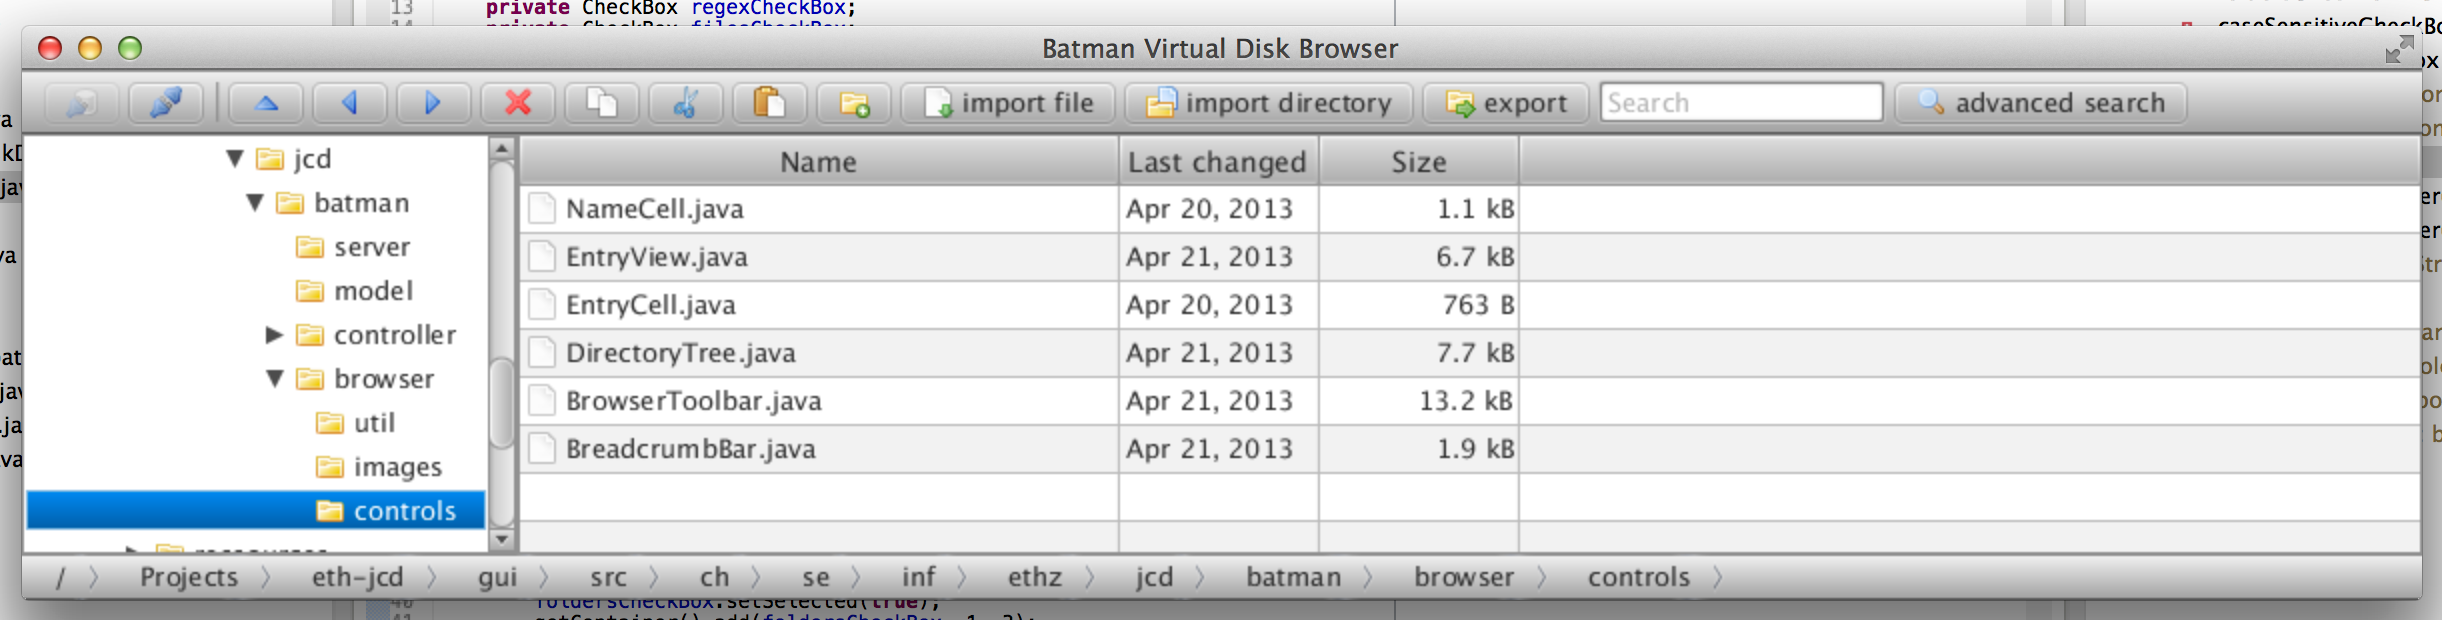
\includegraphics[width=\textwidth]{screen1.png}
    \caption{VFS Browser}
\end{figure}

\subsection{Requirements}
\subsubsection{Platform requirement}
We used JavaFX as our framework to create a desktop application.

\subsubsection{Support all operations from VFS core}
We implemented all operations required by Part 1. This is best seen inside the two interfaces \mono{.server.IRemoteVirtualDisk} and \mono{.controller.TaskController}. The first one is our interface between the client and server. The second interface is the controller (as defined in the MVC Design Pattern) used by the view to execute commands initiated by the user.

\subsubsection{Single and Multiple Selection}
It is possible to execute disk operations on a single disk entry or a list of entries. This can be seen at multiple locations inside our source code. However, the central method involved in this feature is \mono{.browser.GuiState.getSelectedEntries()}.

\subsubsection{Support Keyboard Navigation}
We implemented the following shortcuts. All listed commands are also available as toolbar buttons.
\begin{itemize}
    \item inside the file table:
    \begin{itemize}
        \item \keys{$\leftarrow$} go back in history
        \item \keys{$\rightarrow$} if a folder is selected, go inside it
        \item \keys{$\uparrow$} go to parent folder
        \item \keys{\enter} if a file is selected, open it with default application (tested for Mac OSX and Windows)
        \item \keys{\ctrl + R} rename selected file
    \end{itemize}
    \item in general:
    \begin{itemize}
        \item \keys{\Alt + $\leftarrow$} go back in history
        \item \keys{\Alt + $\rightarrow$} go forward in history
        \item \keys{\Alt + $\uparrow$} go to parent folder
        \item \keys{\ctrl + O} open "Open Disk" dialog
        \item \keys{\ctrl + D} disconnect disk
        \item \keys{\ctrl + C} copy selected disk entries
        \item \keys{\ctrl + X} cut selected disk entries
        \item \keys{\ctrl + V} paste copied/cut entries into current folder
        \item \keys{\ctrl + F} opens the search dialog for the current folder
    \end{itemize}
\end{itemize}

\subsubsection{Mouse Navigation}
As stated above, all keyboard shortcuts can also be executed by clicking on the corresponding toolbar button.

\subsubsection{File-Name Search}
We implemented two kinds of search over disk entry (file or folder) names. The first one is working with simple strings and checks if the given search term is part of a disk entry name. The second one allows to use Regular Expressions (RegEx).

Both searches provide the following settings:
\begin{itemize}
    \item check file names (yes/no)
    \item check directory names (yes/no)
    \item case sensitive / case insensitive search
    \item search inside subfolders (yes/no)
\end{itemize}

Our GUI allows to search directly out of the toolbar. This search sets the settings to a useful default. Otherwise the user can click on ``Advanced Search" and set all the available settings to his choice.

The Search itself is implemented inside \mono{.vdisk.search.VirtualDiskSearch}.

\subsubsection{Bonus: Responsive UI}
All operations are wrapped inside a \mono{javafx.concurrent.Task<V>} and can therefore be executed concurrently. We use this to keep the GUI responsive while operations are executed.

For now we only execute one task at a time. Because of that we have a modal dialog that shows up with a message and a progress bar to give the user feedback about the current task. This dialog only shows up, if the task takes more than five milliseconds. Otherwise the dialog is not visible as the user won't notice the short delay.

The implementation of the tasks can be viewed in our remote controller \mono{.controller.remote.RemoteTaskController}.

\subsubsection{Bonus: Advanced Search}
As already described in ``File-Name Search" we support Regular Expressions and provide additional settings for file-name based search.

\begin{figure}[h]
    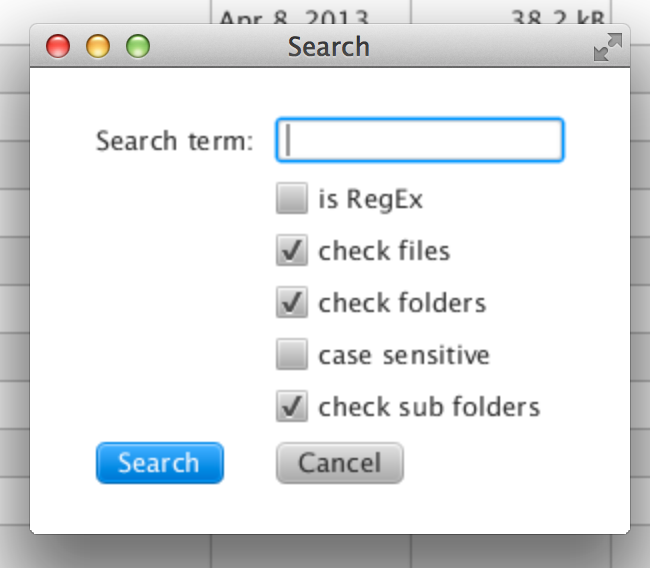
\includegraphics{screen2.png}
    \caption{Advanced Search Dialog}
\end{figure}

\subsubsection{Bonus: Operation Progress Report}
Our modal task dialogs, as described in ``Bonus: Responsive UI", shows additional information to the user. This includes the file on which the current operation is executed, the amount of files already finished and the total count of files to process. A progress bar is used to show the progress graphically as an addition to the raw numbers.

\subsubsection{Bonus: Additional Platform}
We choose JavaFX especially for this feature. JavaFX runs on all major platforms. We developed and tested successfully our VFS Browser on Microsoft Windows and Apple's Mac OSX.

\subsubsection{Additional: Breadcrumbs}
Our VFS Browser includes the breadcrumbs feature at the bottom of the GUI. This shows the current path separated into its parts. By clicking on one of the names the user will jump into the selected directory.

This functionality is well known to Mac OSX and Eclipse JDT users.

\begin{figure}[h]
    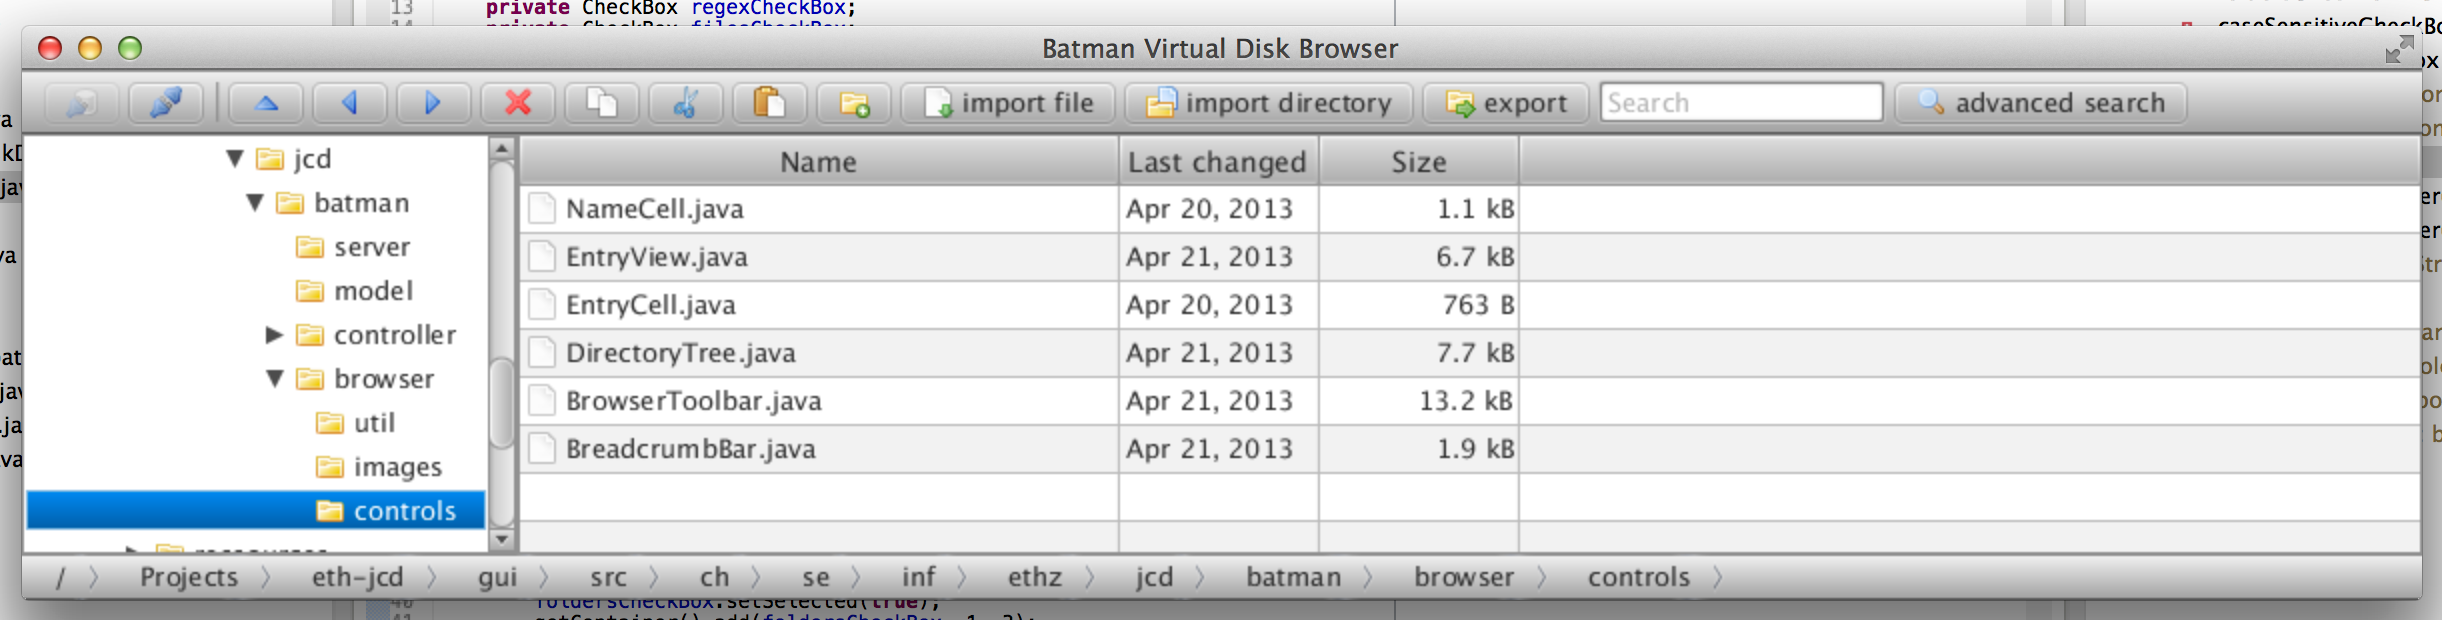
\includegraphics[width=\textwidth]{screen3.png}
    \caption{Breadcrumbs}
\end{figure}

\subsubsection{Additional: Browse History}
We also implemented a history for visited folders. It is possible to go back into previously visited folder and to go forward after that.

\subsection{Design}

\subsubsection{MVC Design Pattern}
Our VFS Browser is heavily based on the Model-View-Controller design pattern. This is for instance reflected in our package names and how the classes inside them are implemented and used:
\begin{itemize}
    \item Model: \mono{.model}
    \item View: \mono{.browser}
    \item Controller: \mono{.controller}
\end{itemize}

\subsubsection{Client-Server-Model}
We implemented our VFS Browser based on the client-server-model. The file browser acts as a thin-client that connects to a server to work with a virtual disk. Therefore the virtual disk is located at a location reachable by the server and doesn't have to be directly reachable by the client.

To connect to the server the user of the client has to provide an URI that represents the location of the virtual disk.

\subsubsection{Controller Factory}
As we use the MVC pattern, we were able to create a view that has no knowledge of the underlying processes and how the operations are executed. Therefore the view does not know that it uses remote method calls to work on a virtual disk that is located at a remote location.

To get the right controller for a virtual disk we use URI addresses that describe the location of the virtual disk that should be opened. The user provides this URI address and the view uses it to get a \mono{controller.TaskController} implementation. To get the right controller for a given URI the view uses our controller factory (\mono{controller.TaskControllerFactory}).

This way it is fairly easy to implement for example a controller that works on a local virtual disk. The developer just has to implement the controller interface (\mono{controller.TaskController}) and add the creation of the controllers to the factory (\mono{controller.TaskControllerFactory}).

Our RMI based controller uses for example the ``batman" scheme (\mono{batman://}). Other schemes can be used for different kinds of controller and ways to connect to a virtual disk.

\subsection{Integration}
We did not have to change any interface inside our core.

While developing the second milestone we discovered three bugs inside the core and fixed them directly.

As ``search" was a new requirement in the second milestone we added the needed and generally useable code to the core, as it belongs logically in there. However, this is purely because of the new requirement.



% PART III: Synchronization Server
% --------------------------------------

\section{Synchronization Server}

The synchronization server allows to work on multiple local virtual disks and keep them in sync by connecting to a central server. The accordingly extended file browser allows the user a simple way to use this new functionality. For the new requirements we extended our server from part two to support a server disk for synchronization proposes.

\subsection{Requirements}

\subsubsection{Important Note}
As we already implemented a client-server-model in part two of this project, we don't really have a ``local disk". Every disk is in some way a remote/server disk. If we talk in the following of a ``local disk" we think about the disk on which the user works. It's also the disk that is always used for all operations without regard if the user is ``online" or ``offline". The ``synchronization disk", or how we call it in our connection dialog, the ``server disk" is the central disk that is used for synchronization while the user is ``online".

% TODO: Remove this text and replace it with actual content
\subsubsection{Creating new account / log in into existing account}
Creating a user and logging in as an existing one is done by using the \mono{.server.ISynchronizeServer} interface. This interface is implemented by \mono{.server.SynchronizeServer}.

The server allows to create unique usernames with a password. The password is saved as a salted hash with the corresponding username inside the \mono{users.data} file. Creating a user on the server side is handled by \mono{.server.SynchronizeServer.createUser(String, String)}.

\begin{figure}[h]\centering
    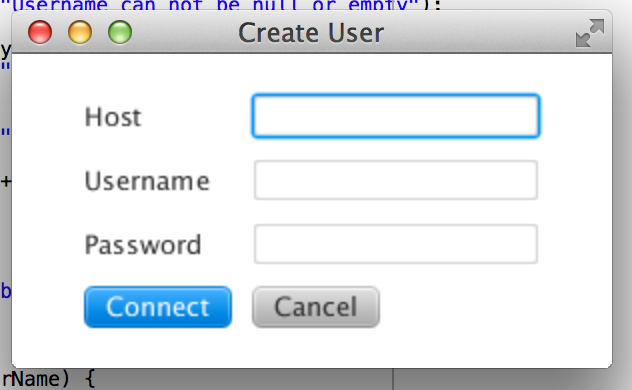
\includegraphics[scale=0.7]{createuser.png}
    \caption{Dialog to create a new user}
\end{figure}

\subsubsection{Go Offline}
We provide the user with a button to go online respectively offline. Either way the user operates on his local disk. If the file browser is in online mode it keeps the local disk synchronized with the remote synchronization disk. If the user connects to the server after being offline the file browser initiates a synchronization right after the connection is established.

This requirement is implemented by \mono{controller.remote.\\ RemoteSynchronizedTaskController.createGoOfflineTask()} and \mono{controller.\\ remote.RemoteSynchronizedTaskController.createGoOnlineTask()}.

\subsubsection{Binding a disk to an account}
This requirement is achieved by linking a local disk to a synchronization disk on a server. If the given disk name already exists on the synchronization server, we link the local disk to it and perform a synchronization. If the name doesn't exists yet it is created and, again, a synchronization is performed.

\begin{figure}[H]\centering
    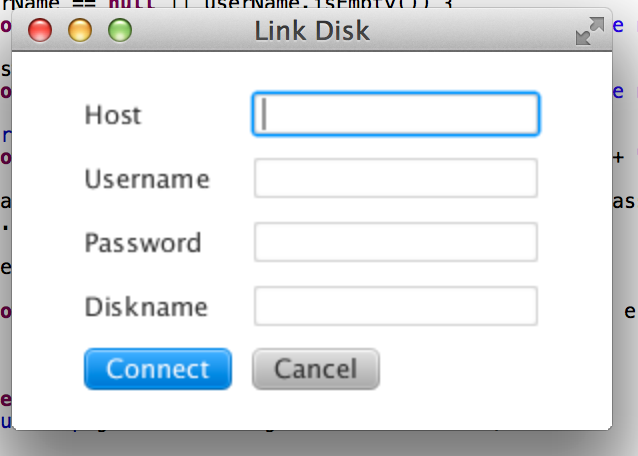
\includegraphics[scale=0.7]{link.png}
    \caption{Dialog to link a local disk to a server disk}
\end{figure}

The provided information about the server is saved on the local disk for future connections. This way the user has only to provide his password the next time he/she goes online.

\begin{figure}[H]\centering
    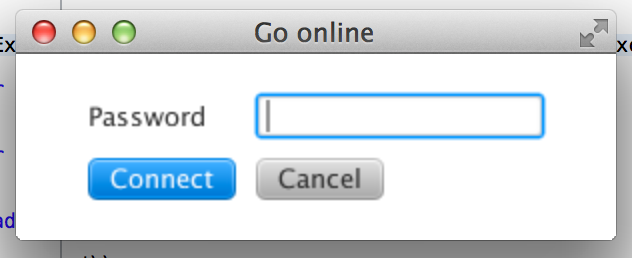
\includegraphics[scale=0.7]{login.png}
    \caption{Login dialog after linking a disk one to a server disk}
\end{figure}

Binding a disk is implemented by \mono{.controller.remote.\\ RemoteSynchronizedTaskController.createLinkDiskTask(String, String, String, String)}.

\subsubsection{Track changes and Synchronize}
The new RMI server interface \mono{.server.ISynchronizeServer} allows to synchronize local disks with a server disk. The logic behind our synchronization process is implemented on the client-side inside \mono{.controller.remote.SynchronizeDisks}.

\subsubsection{Basic: Conflict Resolution}
If the application cannot resolve a conflict it will rename the local version and download the version from the synchronization server. This way the user can decide which one is the right one and no data is lost in any case.

\subsubsection{Advanced: Concurrent Client/Server System}
We implemented both requirements of this advanced requirement. Therefore it is possible to connect with multiple clients to the same synchronization disk and push changes to it. If a change occurs to the server disk, the server notifies all clients of the changes using the \mono{.server.IRemoteDiskClient} interface. After such a notification the client applies the change to the local disk and shows the change in the file browser to the user.

Each client registers his implementation of \mono{.server.IRemoteDiskClient} directly after the server connection is established. The current implementation of the interface is located at \mono{.controller.remote.RemoteTaskController\\.RemoteDiskClient}.

\subsubsection{Additional: Connect directly to a server disk}
Our Open Disk dialog allows to connect directly to a server disk (set ``Connect to" to ``Server"). This will connect the file browser directly to the server disk. It is now possible to do all the normal operations on the disk, without a local copy that is linked to it, and in addition a ``Download disk" button is provided to create a local disk that is in sync with the server disk.

\subsection{Design}

\subsubsection{Client-Server Architecture}
As we already implemented a client-server-architecture in part two, we could just extend the client and server to support synchronization. We provide an all-in-one server class \mono{.server.VirtualDiskServer} to start the local disk server and the synchronization server at once. It is easily possible to only start one of the servers of course. We didn't write classes to start only one of the servers as it won't be used in the given environment.

\subsubsection{Synchronization}
In general the synchronization is done by traversing the file tree to find differences between the synchronization server's disk and the local disk. To help the decision making process we save a timestamp of the last synchronization on the local disk. The following cases exist and were implemented.

\paragraph{A file exists on both disks (same path):} If both files were changed after the last synchronization we have a conflict. This is handled by renaming the local file and downloading the server's version to the local disk. The user has now to decide which one should be kept.

If only one of the two files were changed after the last synchronization, the older one will be replaced with the newer one.

If no changes happened since the last synchronization, nothing has to be done.

\paragraph{A file exists only on one disk:} If the last changed timestamp is older than the last synchronization timestamp the file was deleted and the still existing file on the other disk is deleted. Otherwise the file was created after the last synchronization and is transferred to the other disk while synchronizing.

\paragraph{A folder exists on both disks (same path):} We go inside the folder and check the files.

\paragraph{A folder exists only on one disk:} If the last changed timestamp of the folder is newer than the last synchronization timestamp the folder and it's content is transferred to the other disk.

If the last changed timestamp of the folder is older than the timestamp of the last synchronization we have to check if it contains an object with a timestamp that is newer than the synchronization timestamp. If such an object exists the folder and the found object are transferred to the other disk. If no such object is found, the folder is deleted on the other disk.

\subsection{Integration}
\subsubsection{Documentation}
As we modified some dialogs in the GUI to accommodate the new functionality of the third part of this project, we updated the ``Quick Start Guide" to reflect the changes. All other parts of the documentation were not changed.

\subsubsection{Code Quality}
Some time was taken to change some method names and to fix PMD warnings trough out the code base (part 1-3).

\subsubsection{Changes to part 1}
We used previously reserved metadata space inside our virtual disk to save information about the synchronization disk (host address, username and disk name). Otherwise everything else is the same inside the core.

\subsubsection{Changes to part 2}
We obviously added additional buttons to the file browser GUI. In addition we added controller code to handle the synchronization process and created new code on the server side to provide the needed functionality for the mentioned tasks. In other words, we extended the code base that was built in part two. All functionality that was available in part two is still there with the addition of the new synchronization capabilities.


% PART IV: Quick Start Guide
% --------------------------------------

\section{Quick Start Guide}

\subsection{How to run the CLI}
To run the Command Line Interface just run \mono{.cli.Main.java}. A host system path is a path that is valid for the host system. A virtual disk path is a valid path for the virtual disk.

\subsection{Commands}
Following a list of available commands with a description what they do.
\begin{description}
    \item [stop] Stops the CLI and shuts down the application. Example: \mono{stop}
    \item [create] Takes a valid file path (host system) where it will create a new, empty virtual disk. Example: \mono{create /home/user/test.vdisk}
    \item [destroy] Takes a valid file path (host system) where a virtual disk is located. After successfully checking for the magic number it will delete the disk from the host's system. Example: \mono{destroy /home/user/test.vdisk}
    \item [load] Takes a valid file path (host system) where a virtual disk is located. Will load the given file as a virtual disk. Example: \mono{load /home/user/test.vdisk}
    \item [unload] Unloads the currently loaded virtual disk. Example: \mono{unload}
    \item [ls] Takes an \textit{otional} argument with an absolute or relative path (virtual disk). Will print out all children (files and directories) inside the given path or for the current location. Example \mono{ls /}
    \item [mkdir] Takes an absolute or relative path (virtual disk) and creates a directory at the given location. It is possible to pass ``-p" as the first argument and a path as the second one, in this case it will create all needed directories to satisfy the given path.\\ Example: \mono{mkdir -p /test/some/stuff} will create the directories /test, /test/some and /test/some/stuff.
    \item [cd] Takes an absolute or relative path (virtual disk) as its argument. Changes the current directory to the given path. Example: \mono{cd /test/some}
    \item [size] Takes an \textit{optional} relative or absolute path as its argument. Returns the size of the object represented by the given path (or the size of the current one, if no path provided). Example: \mono{size /test}
    \item [query] Takes ``occupied", ``free" or ``total" as its first argument. Example: \mono{query total}
    \begin{description}
        \item [occupied] Shows the amount of used space inside the virtual disk
        \item [free] Shows the amount of not used space inside the virtual disk
        \item [total] Shows the size of the disk on the host system
    \end{description}
    \item [delete] Takes an absolute or relative path to a directory or file inside the virtual disk. Deletes the given object. Example: \mono{delete /test}
    \item [move] Takes two absolute or relative paths (virtual disk). The first being the source and the second being the target. Moves the source file or directory to the given target. Example: \mono{move /test/some/file /test/} would move the file ``/test/some/file" into the directory ``/test/" (resulting in a new file ``/test/file")
    \item [copy] Takes two absolute or relative paths (virtual disk). The first being the source and the second being the target. Creates a copy of the source at the given target location. Example: \mono{copy /test/some/file /test/file}
    \item [import] Takes two absolute or relative paths. The first one being a source (host system) and the second one being a target (virtual disk). Will import the file or directory from the host system into the given target inside the virtual disk. Example: \mono{import /home/user/movies/awesome.avi /awesome.avi}
    \item [export] Takes two absolute or relative paths. The first one being a source (virtual disk) and the second one being a target (host system). Exports the given source file or directory into the given target. Example: \mono{export /awesome.avi /home/user/movies/}
\end{description}

\subsection{How to use the VFS Browser (second and third milestone)}
As we implemented the second milestone based on the client-server-model there are some steps needed to get it running.

In general the following steps are required:
\begin{enumerate}
    \item start RMI Registry (\mono{rmiregistry}/\mono{rmiregistry.exe})
    \item start our server (\mono{.server.VirtualDiskServer})
    \item start the GUI (\mono{.browser.Main})
    \item connect to the server
\end{enumerate}

\subsubsection{Start rmiregistry}
\mono{rmiregistry} needs to know where the compiled \mono{.class} files are kept and therefore it is important to set the \mono{CLASSPATH} environment variable correctly. This variable has to include the path to both bin folders (\mono{core/bin} and \mono{gui/bin}) and the file path to the JavaFX JAR file (\mono{jfxrt.jar}).

On our Mac OSX machine we used the following shell script to start the \mono{rmiregistry} (paths must be modified accordingly):
\begin{lstlisting}[language=bash,breaklines=true,frame=single]
export CLASSPATH="/Users/groggi/Projects/eth-jcd/gui/bin:/Users/groggi/Projects/eth-jcd/core/bin:/Library/Java/JavaVirtualMachines/jdk1.7.0_17.jdk/Contents/Home/jre/lib/jfxrt.jar"


/Library/Java/JavaVirtualMachines/jdk1.7.0_17.jdk/Contents/Home/bin/rmiregistry
\end{lstlisting}

On our Windows machine we used the following batch script to start the \mono{rmiregistry} (paths must be modified accordingly):
\begin{lstlisting}[language=bash,breaklines=true,frame=single]
set CLASSPATH=C:\Users\Benji\Documents\GitHub\eth-jcd\gui\bin;C:\Users\Benji\Documents\GitHub\eth-jcd\core\bin;C:\Program Files\Java\jdk1.7.0_17\jre\lib\jfxrt.jar

"C:\Program Files\Java\jdk1.7.0_17\bin\rmiregistry.exe"
\end{lstlisting}

\subsubsection{Connecting disk}
In comparison to the version of part 2 we now provide a simpler interface for connecting to a local disk. The user has to provide the host address (e.g. \mono{localhost}) of the server and the path on the host system where the disk is located or should be created (e.g. \mono{/tmp/mydisk.vdisk}).

\begin{figure}[H]\centering
    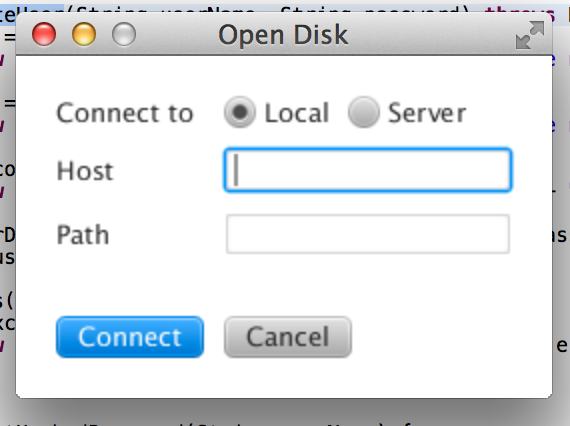
\includegraphics[scale=0.7]{local.png}
    \caption{Dialog to connect to a local disk}
\end{figure}

The option ``Connect to Server" allows to connect directly to a synchornization disk. This connection allows to download the disk or work directly on it without a local copy.

\begin{figure}[H]\centering
    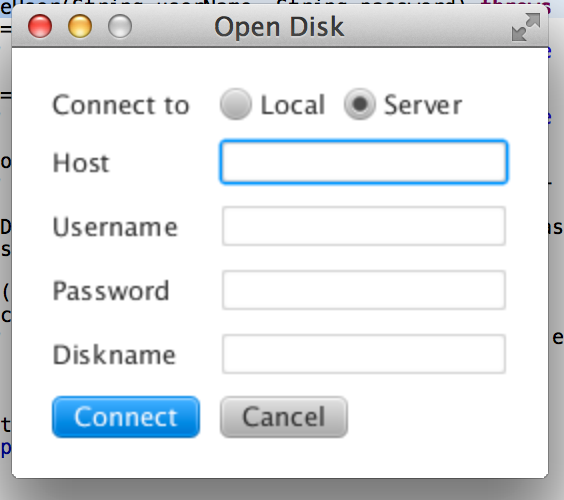
\includegraphics[scale=0.7]{server.png}
    \caption{Dialog to connect to a synchronization disk}
\end{figure}


\subsubsection{Starting the GUI}
\paragraph{Start synchronization server on localhost:} Follow the steps described in ``How to use the VFS Browser (second and third milestone)" and it's subsections.

\paragraph{Create account on synchronization server:} In the file browser GUI click on ``Create User". Use \mono{localhost} as your ``Host" and choose a username and password.

\paragraph{Create two VFS disks and link them to the new account:} Open a second file browser GUI for the second disk. Do the following in both GUIs: Click on the first toolbar button (``connect"), select ``Local", use \mono{localhost} as the ``Host" and write a valid file path to the location where the new disk should be created.

After you created the disk click on ``Go online" to create a connection with a synchronization disk. In the dialog write \mono{localhost} as your host, put in the previously created username and password and choose a name for the synchronization disk. Repeat this with the second disk (second file browser window).

\paragraph{Import a directory:} Click on ``Import directory" in the toolbar and select the directory to import.

\paragraph{Dispose Disk 1:} Open the file browser for the disk you choose as disk 1 and click on the ``Delete disk" button inside the toolbar.

\paragraph{Export the directory:} Select the directory to export inside the file browser with a left mouse click and click after that on ``export".

\paragraph{Stop synchronization server:} Close all file browsers and just kill the RMI Registry and the running \mono{.server.VirtualDiskServer}.


\end{document}
